%\documentclass[times, 10pt, twocolumn]{article}
%\documentclass[conference,final]{IEEEtran}
     
\documentclass{rspublic}   

%------------------------------------------------------------------------- take
%the % away on next line to produce the final camera-ready version
%\pagestyle{empty}

\usepackage[utf8]{inputenc}
\usepackage{graphicx}
\usepackage{url}
\usepackage{float}
\usepackage{times}
\usepackage{multirow}
\usepackage{listings}
\usepackage{times}
\usepackage{paralist}
\usepackage{wrapfig}
\usepackage[small,it]{caption}
\usepackage{multirow}
\usepackage{ifpdf}
\usepackage{subfigure}
%\usepackage{subfig}
%\usepackage[pdftex]{graphicx}
%\usepackage{harvard}
%\usepackage{pdfsync}

%Bibliography     
\usepackage{natbib}                
\usepackage{listings}
\usepackage{keyval}
\usepackage{color}
\definecolor{listinggray}{gray}{0.95}
\definecolor{darkgray}{gray}{0.7}
\definecolor{commentgreen}{rgb}{0, 0.4, 0}
\definecolor{darkblue}{rgb}{0, 0, 0.4}
\definecolor{middleblue}{rgb}{0, 0, 0.7}
\definecolor{darkred}{rgb}{0.4, 0, 0}
\definecolor{brown}{rgb}{0.5, 0.5, 0}
\definecolor{orange}{rgb}{1,0.5,0}

\lstdefinestyle{myListing}{ frame=single, backgroundcolor=\color{listinggray},  
  %float=t,
  language=C,       basicstyle=\ttfamily \footnotesize, breakautoindent=true,
breaklines=true tabsize=2, captionpos=b, aboveskip=0em,
  %numbers=left, numberstyle=\tiny
}      

\lstdefinestyle{myPythonListing}{ frame=single,
backgroundcolor=\color{listinggray},  
  %float=t,
  language=Python,       basicstyle=\ttfamily \footnotesize,
breakautoindent=true, breaklines=true tabsize=2, captionpos=b,  
  %numbers=left, numberstyle=\tiny
}

\title[Understanding Performance Implications of Distributing Data for
Data-Intensive Applications]{Understanding Performance Implications of
Distributing Data for Data-Intensive Applications}


\author[Miceli, Miceli, Rodriguez-Milla, Jha]{ Christopher Miceli$^{1}$,
Michael Miceli$^{1}$, Bety Rodriguez-Milla$^{1}$, Shantenu Jha$^{1,2,*}$ \\
\small{\emph{$^{1}$Center for Computation \& Technology, Louisiana State
University, USA}} \\  \small{\emph{$^{2}$Department of Computer Science,
Louisiana State University, USA}} \\ {\footnotesize {\hspace{0.0 in}
$^*$Corresponding Author sjha@cct.lsu.edu}} }

%\date{}

\def\acknowledgementname{Acknowledgements} \newenvironment{acknowledgement} 

% {\section*{\acknowledgementname}%\parindent=0pt% }

\newif\ifdraft \drafttrue \ifdraft \newcommand{\fixme}[1]{ { \bf{ ***FIXME: #1
}} } \newcommand{\jhanote}[1]{ {\textcolor{red} { ***Jha: #1 }}}
\newcommand{\micnote}[1]{ {\textcolor{blue} { ***Michael: #1 }}} 
\newcommand{\betynote}[1]{ {\textcolor{orange} { ***Bety: #1 }}}
\else
\newcommand{\jhanote}[1]{} \newcommand{\micnote}[1]{}\newcommand{\betynote}[1]{} \newcommand{\fixme}[1]{}
\fi

\begin{document} \maketitle

\micnote{This can't be more than 200 words.  The summary should be concise and
informative.  It should be complete by itself, and must not contain references
or unexplained abbreviations.  It should not only indicate the general scope of
the article but also state the main results and conclusions.  Please note that
footnotes are not used.}

\begin{abstract}{data-intensive computing, distributed computing, cloud
computing, grid computing} Grids, clouds and cloud-like infrastructures
are capable of supporting large problems.  While the capability of these
systems is great, unique performance issues appear as data-sets become
extremely large.  As the volume of data increases, scalable placement
and management techniques are required.  Often, it is hard to predict
where to place data to where it minimizes data transfer.  This paper
uses two techniques to manage data placement.  One focuses on data
placement and the other on worker placement.  Distributed Filesystems
(DFS) focus on data placement.  They simplify the management of
distributed data by providing a single access protocol and a common
name-space, and encapsulating data placement issues.  Although this
simplifies the management of data, there are potential performance
trade-offs.  Users can no longer control data placement, which possibly
has performance implications.  Another approach is for the work to be
aware of the data and adjust accordingly. This technique can move the
work to the data or vice-versa has different performance issues than a
DFS.  The goal of this paper is to understand techniques for
distributing data in a distributed environment and understand
performance issues associated with these techniques.\micnote{conclusion
needs to go here *can be 12 words*}\end{abstract}

\section{Introduction} Data-intensive computing is a fast growing area
of computer science.  A good example of this is Google, which processes
around 20 petabytes of data per day ~\citep{google}, and trends show
continuing growth.  It has become very important that a distributed
application developer takes precautions when placing, scheduling, and
managing large volumes of data.  Careless placement can adversely affect
system performance greatly.  It is decisive then to determine whether to move input data to the computational resource, or the computational workload to the input data.
There are two ways to handle this issue, with 
distributed filesystems, which focus on data placement, or with the use of an
intelligent framework, which focuses on worker placement. 

Distributed filesystems (DFS), motivated in part by
developments in cloud computing, are useful and effective tools to consider for
data-intensive scientific applications. A DFS controls the data placement and provides
a uniform interface for accessing files on multiple hosts.
Frequently, there is more than
one copy of the input data for fault-tolerance reasons, consequently, the added
issue of deciding between the two or more replicas becomes relevant.
While a DFS removes the responsibility of replica management and data
server placement, the abstraction often increases the difficulty in
determining where in the DFS the data is being stored.  This
puts pressure on a DFS's protocols and internal algorithms to perform
well.  Despite this, the DFS replication may alleviate this issue by
placing replicas in locations where computational resources reside. 
A downfall of DFSs is the inability to make the decision of whether to move
the input data, or the computational workload.  It can only
focus on minimizing poor data management. The most common parameters
in determining the performance of using a DFS are the performance
overhead compared to a normal local filesystem, number of replicas of
each datum/file, and the number of servers. In our experiments, 
we use the stable open source
distributed filesystem CloudStore (formerly KFS), which is written in
C++ released under the Apache License Version 2.0.  It is inspired by
the highly successful Google Filesystem, GFS ~\citep{cloudstore_web}, 
which is closed source and
unavailable for research.  CloudStore was chosen for its
 high performance focus, C++
implementation, and its source code availability. It
also provides a means to automatically replicate data on 
different hosts to provide
efficient data access and fault tolerance.  

Our intelligent framework method differs from a DFS in that it
determines where data is and where the work should go. 
Determining data location can be as simple as
looking at the IP address of the worker and seeing geographically where
it is located or as complicated as using network analyses tools to
determine the optimal data transfer minimization time. 
For this method, we use gridFTP, a tool that is used to transfer
files across machines in a grid.  It is
specifically designed for high-bandwidth networks. GridFTP  is provided by
the Globus Toolkit, an open source software toolkit
released under the Apache License version 2.0.  Globus provides tools used
to create and manage grid infrastructures. 

In this paper, we provide some initial approaches to answer
 ``To distribute or not to distribute data, is the question''. 
 Our research focuses on understanding the performance trade-offs
  of a DFS compared to ''regular''
distribution and placement techniques, as well as more advanced
intelligent distribution methods and finding how
they handle different data-sets and what there performance patterns
are.  This paper also aims to determine
how sensitive the performance is in the context of a real data-intensive
distributed applications.

\section {Methodology (change to a better title)}
We use an application based upon a
grid-enabled All-Pairs abstraction in SAGA (Simple API for
Grid Applications, see Sec. \ref{Sec:SAGA}). This abstraction applies an operation on two
data-sets such that every possible pair containing one element from the
first set and one element from the second set has some operation
applied to it.~\citep{Interop, AllPairs}  Essentially, All-Pairs is a
function of two sets, $A$ and $B$, with number of elements $m$ and $n$, respectively, which creates a matrix $M$. Each element $M_{i,j}$ is the
result of the operation $f$ applied to the elements $A_i$ and $B_j$.
\begin{eqnarray}
 AllPairs(A, B, f) & \rightarrow & M_{m \times n}, \\
\mbox{where} \quad M_{i,j} & = & f(A_{i},B_{j})
 \end{eqnarray}
 
The result of this application is stored in a matrix.  The
application spawns distributed jobs to run sets of these pairs.  The
problem becomes determining which pairs to put into a set, and with
which distributed resource to run that set.  If transferring data to the
job takes too long, we spend more time on data management than
computation.  There may be a resource capable of the work that may be
slower than others, but network-close (able to be accessed in a
relatively quick manner via the network supporting the distributed
system) enough to the data to make up for its lack of computational
ability. 

Examples of problems that
fall into this category are image comparison for facial recognition, and
genome comparison.  This paper uses genome comparisons to find the best
matching gene in a genome. \micnote{I think we should have a small
graphic here to show the matrix and how it works}

%There are at least two types of data-intensive applications: the first
%where the actual data generated is large; the second type is where the
%data generated is small, but the volume of data on which computation
%occurs is very large.  The application we used, has relatively small
%input and relatively small output, but the manner of processing causes
%many data reads.  This type of application can be classified as having
%a large data throughput.  \jhanote{Can you elaborate on different
%types of data-intensive applications?  What kind is an ImageMagic
%based application?}

Our genome comparison application can be classified as having a large
data throughput, as, even though it
has large input $O$(GB) and relatively small output $O$(KB), the manner of 
processing causes many data reads.  To
handle seamlessly the DFS and gridFTP based data stores, and to 
facilitate usage on clouds and grids, the application
uses the Simple API for Grid Applications (SAGA) ~\citep{saga_web}.
This allows the same exact application to be used for all of our
experiments.  

\section{SAGA} \label{Sec:SAGA}

\section{Performance Measurement and Analysis}
We developed three types
of experiments in order to compare distributed filesystems with manual
file management. Some of the questions we try to answer are, 
does a distributed filesystem grow more slowly than
manual placement of data?  When manually handling data, what are the
advantages of being able to move work to data to the work? For this, we find 
the time to completion $t_c$, which is a function of pre-processing time $t_x$, I/O time $t_{I/O}$, which is the time it takes to read and write files, and the time to compute $t_{compute}$, which is the time it takes for genomes to be compared, i.e.,
\begin{equation}
t_c = t_x + t_{I/O} + t_{compute}.
\end{equation}
We focus on three variables to measure $t_c$:  degree of distribution, data
dependency, and workload.
\betynote{We should find variable names for the 3 variables, like $D_d$, w
 for workload, etc, define them and add that to the $t_c$ equation as $t_c(var1, var2, var3) = t_x()$...}
\betynote{check name, role, text of $t_x$}

\subsection{Experimental Configuration}

As explained before, for our experiments, we used an All-Pairs
 implementation that utilises SAGA. Our specific
implementation is given via an xml configuration file. Such file, defines 
the location of
the data that comprises the two input sets, the grouping of pairs from
these sets into sets to be provided to the compute resources, and the
available machines that will perform the operation on these sets of
pairs.  The application takes these sets of pairs and maps them to a
computational resource dynamically at run-time.

Furthermore, variables external to the All-Pairs implementation also
influence experimental results. The following experiments can be
completely described by a tuple of the following form
 \begin{equation}
(d, c, dc, fs, m,r),
\end{equation}
where $d$ is the total amount of data in each element, or file, of a set (i.e., $d=\mbox{\textit{chunk} size}$); 
$c$ is the number of elements in each set (i.e., number of files per set); \betynote{most of the graphs don't talk about $c$, either we say that before hand, and erase $c$ in here, or we add c to all graphs, most of the cases  $c= 8$}
$dc$ is a comma separated list of the following
form: $X(A1, A2)$ where $X$ is a shorthand for the computational resource, $A1$
is whether computational resource $X$ assisted calculations, and $A2$ is
whether computational resource $X$ assisted in data storage; 
$fs$ is the type of filesystem used;
$m$ is the method used to access that filesystem; and
$r$ is the amount of replication utilized in the experiment. For example, 
 \begin{equation}
(287 \mbox{MB}, 8, E(Y, N), P(N, Y), \mbox{CloudStore, Direct}, 1),
\end{equation}
shows that each element of a set is 287 MB in size; we have 8 elements in each set;  the computational resource $E$ does calculations, but does not have data stored, while computational resource $P$ does not calculate, but stores the data; the filesystem used is CloudStore, it directly access the files, and we have a replication factor of 1 for our data.

In our experiments, we have three $(fs, m)$ configurations, and few $X$ configurations. Our $(fs, m)$ configurations are $LL=(\mbox{local, local})$, $LG=(\mbox{local, gridFTP})$, and $CD=(\mbox{CloudStore, direct})$.\betynote{Explain what all they mean, and find a better name other than f1, f2, f3.} Our $X$ configurations are, for one machine, $A1(Y,Y)$, where resource $A1$ has both the data and the computing. For two machines, we have four configurations. The first one is $C1=A1(Y, Y), A2(N, N)$, where $A1$ has the data and runs all the jobs, while $A2$ is added in our xml file, but does not participate. In the local case, this is equivalent to our one machine case, but not when we use CloudStore, as it also contributes to $t_x$. In the second one, $C2=A1(Y, N), A2(N, Y)$,  $A1$ computes with the data stored at $A2$, here, $A2$ does no computation. The third one, $C3=A1(Y, Y), A2(Y, N)$, has the data in $A1$, but computes in both $A1$ and $A2$ machines. In the fourth configuration, $C4=A1(Y, Y), A2(Y, Y)$, we distribute the data into two machines, half of the files go to $A1$, and half go to $A2$, both machines compute. For three machines, we have a unique configuration of  $A1(Y, Y), A2(Y, N), A3(Y, Y)$, where the data is distributed in all three machines, and all of them compute. We run our experiments in the grid LONI (Louisiana Optical Network Initiative).

As described above, the All-Pairs implementation used for our
experiments has a fixed distribution of data, fixed available
computational resources, and fixed sets of pairs to operate with.
These variabilities listed above will be manipulated to determine causes
for different I/O complexities observed in an attempt to build an
understanding of issues that arise when utilising data-intensive
applications.

\fixme{Define C as  tuple of (i) Chunk Size (number), (ii) Infrastructure,
(iii) FS configuration, (iv) Data-Access protocol.}
Mention for CloudStore we also need to include a replication factor. \betynote{We have to specify replication factor for the local, gridftp case}



\subsection{Experiment I: Baseline Performance}
 In the first experiment, we have no actual
operation begin applied on the pairs, this is, $t_{compute}=0$.  
The reasoning behind this is to
evaluate data dependencies without the added variable of computation. 
We run the SAGA-based All-Pairs application on one, two, and three
unique machines on a grid (LONI),
 without any specific data placement
strategy; also, no replication or fault-tolerance takes place.  The
application sequentially assigns sets of pairs to the first available
computational resource.  All data is accessed via the gridFTP protocol.
An important fact to notice is the essentially random mapping of data
sets to computational resources based on availability.  This is to mimic
a naïve data-based application. In figure \ref{Fig:ExpIConventionalLocal}, we show our results for one and two machines (Figs. \ref{Fig:ExpIConventionalLocal:a}, and \ref{Fig:ExpIConventionalLocal:b}, respectively). In figure \ref{Fig:ExpIConventionalLocal:a}, our local experiments, we see that \betynote{WHY is t(287, 8) $<$ t(144,16)} \betynote{Graphs need and (a) or (b), upper left corner, depending if there are two plots, left or right.} 
%Figure 1
\begin{center}
\begin{figure}[ht]
\subfigure{
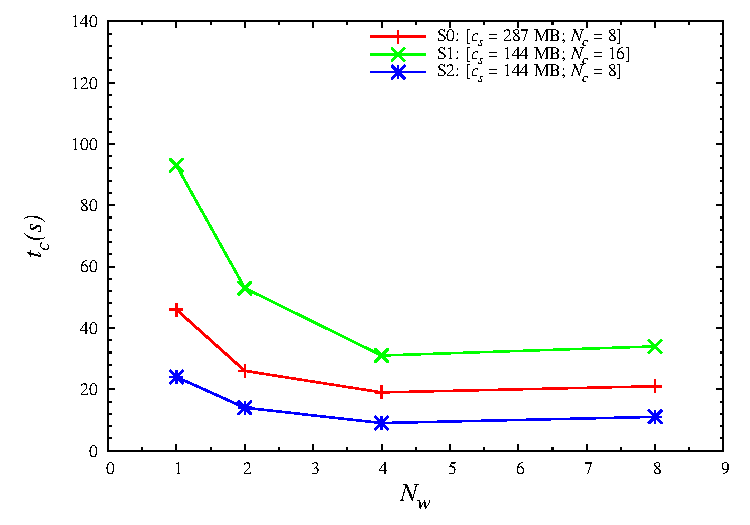
\includegraphics[scale=0.55]{data/graphs/LocalFigure}
\label{Fig:ExpIConventionalLocal:a}
}
\subfigure{
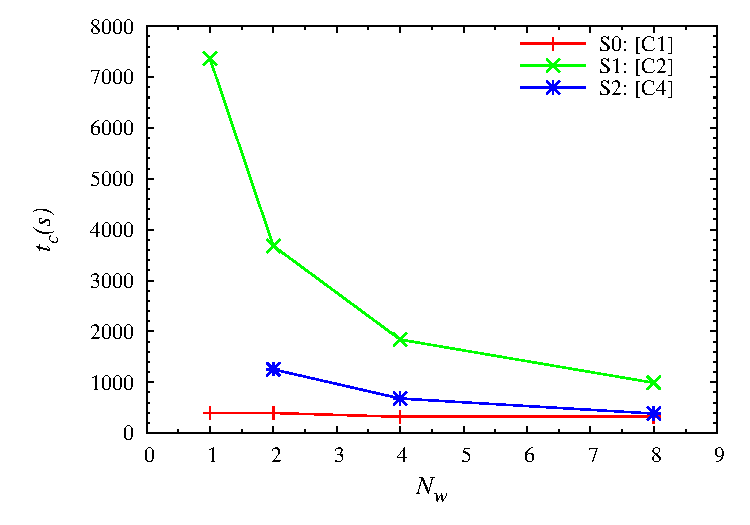
\includegraphics[scale=0.55]{data/graphs/ConventionalFigure}
\label{Fig:ExpIConventionalLocal:b}
}
\caption{\textit{Performance results for All-Pairs using GridFTP for
file reads being compared to a completely local run.}}
\label{Fig:ExpIConventionalLocal}
\end{figure}
\end{center}

\subsubsection{With Computation} 
The previous experiments 
In order to properly evaulate all properties of a data-intensive
application in practical use, we added the actual genome compare
computation.  The complexity added that is necessary to capture to is
the scaling of computation time when multiple computational resources are
coallocated.

%Bety's graph goes here
\jhanote{We need data for compute (comparision) and I/O (only) for
different data-set sizes} \micnote{We need data for three and four
machines (just one graph going from 1 machine to four machines}

%Staging experiment
\subsection{Experiment II: Staging}
The second experiment is similar to the
first, except the All-Pairs application observes the data's location
before determining whether or not to assign a certain set of
data-dependent computation to an idle job.  Inspired by earlier
work~\citep{netperf}, this version of the application performs an extra
step during application startup that approximates the performance of the
network by pinging the hosts that may be be either a computational
resource or a data store and then  assembling a graph structure.  This
data structure is utilised when the time comes to map an idle worker to
an unprocessed portion of compuational pairs.  This changes the
first-available compuational resource assignment mechanism descrbied in
the first experiment.  Though ping is not very sophisticated in terms of
describing a network's behavior, it is a first-approximation to
performance model aware data-placement strategy.  This approach knows
where the files are located and then determines whether to move the work
to where the data is, or move the data to the work.  \jhanote{Data-aware
placement is also required, i.e., managing location of files.}  

We introduce the idea of network-closeness.  A network-close data-set
takes a small amount of time to transfer to the work location.  A
network-far data-set is just the opposite.  A network-far data-set takes
a long time to transfer to the work location.  If there is an
unprocessed data-set collocated or network-close with the job, then the
assignment of that worker to that data-set would have benefits.  If
there is no unprocessed data-set that is network-close to the job, still
we assign data that may be network-far, in case the network-close job
failed or there is no available jobs network-close to the data-set.
%Figure 2
\begin{center}
\begin{figure}
\subfigure{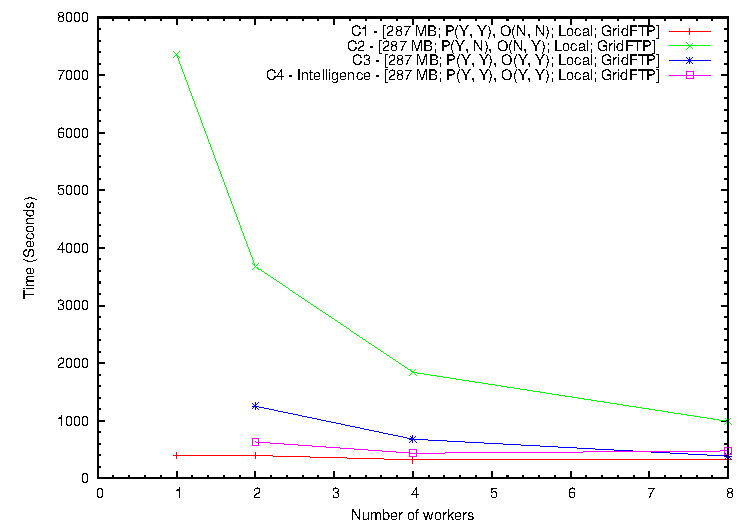
\includegraphics[scale=0.55]
   {data/graphs/IntelligentVsConventionalFigure}}
\subfigure{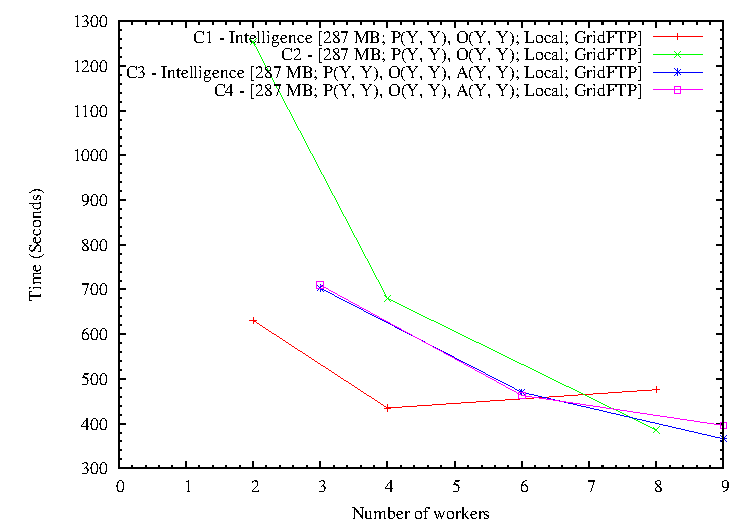
\includegraphics[scale=0.55]
   {data/graphs/IntelligentFigure}}
\caption{\textit{The figure on the left demonstrations improved
performance with minimal network awareness while the figure, while the
figure on the right demonstrates less performance improvement when more
resources are involved.}}
\label{experiment2}
\end{figure}
\end{center}

Some remarks about performance: the overhead of intelligence includes
all time spent pinging hosts and building the graph data structure.  The
total time spent this overhead was negligible at approximately two
seconds per application run.

\subsection{Experiment III} The third experiment provides information
into CloudStore's performance in handling data locality issues.  The
same All-Pairs application as in Experiments 1 and 2 is used, except all
data is stored on the distributed filesystem CloudStore under various
configurations.  Some variables of importance include number of data
servers that store data, replication value for data in these data
servers, and as above, placement and number of computational resources.
All read and writes also utilise the distributed filesystem.  
%Figure 3
\begin{center}
\begin{figure}
\subfigure{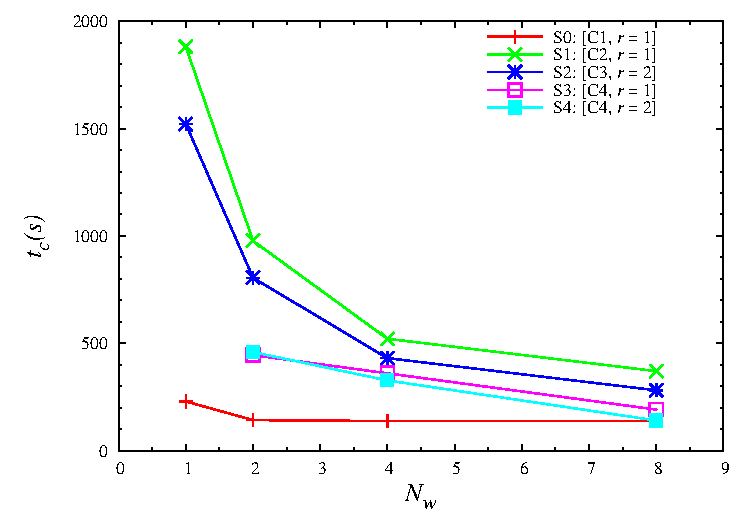
\includegraphics[scale=0.55]
   {data/graphs/CloudStoreFigure}}
\subfigure{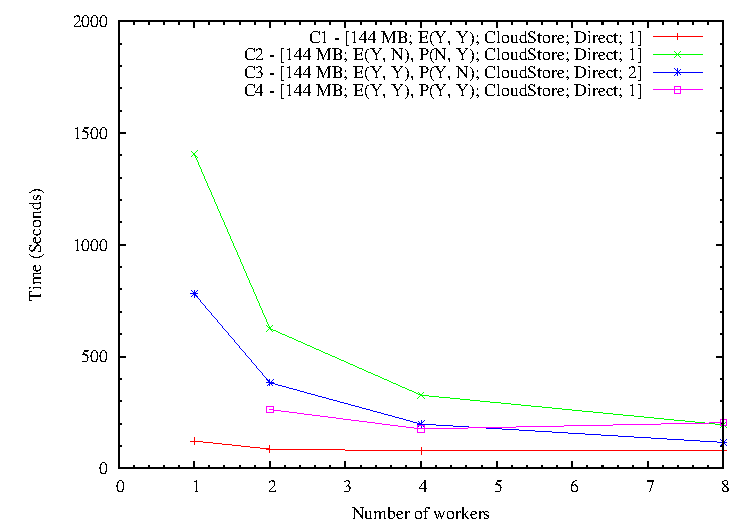
\includegraphics[scale=0.55]
   {data/graphs/CloudStoreNoComputeSmallerDataSet}}
\caption{\textit{Comparison of CloudStore using the All-Pairs
application for different set sizes.}}
\label{experiment3}
\end{figure}
\end{center}

\subsubsection{with Computation}  \micnote{Sentence about c2 and c3:  On
the left hand side of Figure 3, line C2 has data distant from the
computation.  Line C3 has data mixed with some resources.  They follow
the same curves with line C3 having speed improvements.} As done above
for the first experiement, for completion with have attempted to capture
how compute time scales under these configurations.
%Figure 4
\begin{center}
\begin{figure}
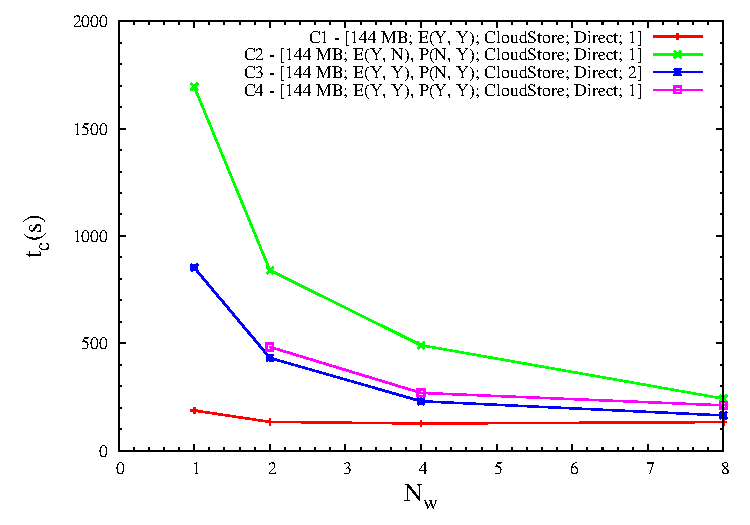
\includegraphics[scale=.75]{data/graphs/CloudStoreCompute}
\caption{\textit{Comparison of CloudStore using the All-Pairs
application with actual computation.}}
\label{experiment3compute}
\end{figure}
\end{center}

\section{Analysis}

Overall, the use of CloudStore decreases the time to completion
($t_c$) compared to the intelligent and the local approaches. Our
simple intelligent approach did not performed as well as CloudStore, but
works better than the local tests. For the parameters we used, the
introduction of more workers, up to 8 in our case, decreases the time of
completion; however, for the case of a single machine performing as both
master and workers, we hit an I/O bound, probably caused by the network.
For all of our approaches, GridFTP, Intelligent, and CloudStore, we find
the time to completion for three cases: a single machine is the master
and the workers, one machine does the computing while another has the
data stored, and the case when we spread the data into both machines,
while both of them compute.  In all of our three approaches, the case of
a single machine, shows the least $t_c$. In the case of two machines,
having the data in one, and computing in the other one, increases the
time to completion. By splitting the data in both of the machines, and
computing in both, we decrease $t_c$. We then added another case, all
the data in each of machines, and computing in both. This decreases the
time even further, but not to the point of the local computations;
perhaps, all the approaches are not guaranteed to use the data in the
machine the job is being run, even thought the data is in both machines.

???For our three cases,  $t_c$ may be bounded, and decrease to $t_c$(single machine) as  the number of workers ($N_w$) increases, up to a critical $N_w$, after which $T_c$ will increase due to worker coordination overhead.





\section{Conclusion} Our results show that a DFS greatly changes the
performance of a distributed application in a positive manner.  Our
experiments that utilised the DFS to access and store data outperformed
their gridFTP counterparts by an order of magnitude in most cases. Our
results also indicate that the DFS scales better as file sizes and
number of files grow, although both seem to scale linearly.  Before any
conclusions may be drawn, there are issues that need to be addressed.
Our application utilised SAGA to access DFS based and gridFTP based
files.  Although there is clearly a SAGA induced overhead, this overhead
is constant.  \jhanote{ We need to discuss performance issue: Ole has
performance numbers that contradict this, i.e., the overhead that SAGA
introduces for file/gridFTP is very small compared to native globus
calls.  This may be due to SAGA's adaptive nature, where lots of
computation is spent determining how to make a distributed call.  Other
reason's may be the gridFTP SAGA adaptor being separated from the
application, being able to make only general decisions, allowing no
performance tweaks.  Accessing files through this abstraction
with gridFTP seemed to perform sub-optimally in comparison to using the
globus tools directly.} In addition, we were unable to utilise our
entire distributed system, using at most 8 jobs to handle our work.
With a replication level of two in the DFS, data was almost certainly
co-located with the computational resource.  In the second experiment,
utilizing information from first staging the network did improve upon
the results of the naive first experiment, but still did not approach
the DFS's performance levels.

Distributed filesystems are important abstractions for a data-intensive
distributed application developers to consider.  It also appears that
staging is worth the time required to build a graph representing the
network.  Also to note, the second experiment is also naive in the way
that it attempts to optimise data and work assignments.  Our staging
only performed pings, not data transfer trials or reliability tests.  A
job could have low latency, but poor bandwidth.  Perhaps CloudStore's
performance can be attributed to recent work that has shown that data in
large scale distributed applications tends to be accessed together,
despite being seemingly unrelated in the input data-set.  Such
correlation in data-access has been observed elsewhere, and specific
abstractions to support the access of ``aggregation of such files'' has
been referred to as a filecule, an application specific group of
files~\citep{filecule}.  Attempting to determine if analogous
abstractions could enhance performance for the All-Pair application
could be interesting.  In a DFS, however, if the data store is also
capable of data processing, then the DFS is placing commonly used files
together on machines needing them for work; in essence, the DFS is
finding these groups for the developer.  The fault tolerance, for which
distributed filesystems are already well renowned for, also has added
benefits to grid application developers in terms of performance.  The
distributed application does not have to be aware of where data has been
copied to previously when assigning work; the distributed filesystem
uses the best replica when data is being accessed.

\fixme{This should be changed to be appropriate \bf{**Shantenu**}}
{\bf Acknowledgment:} Important funding for SAGA has been provided by
    the UK EPSRC grant number GR/D0766171/1 (via OMII-UK) and HPCOPS
    NSF-OCI 0710874. SJ acknowledges the e-Science Institute,
    Edinburgh for supporting the research theme, ``Distributed
    Programming Abstractions'' and theme members for shaping many
    important ideas. This work has also been made possible thanks to
    the internal resources of the Center for Computation \& Technology
    at Louisiana State University and computer resources provided by
    LONI. 

%\bibliographystyle{IEEEtran}
\bibliographystyle{kluwer} 
\bibliography{data_intensive_paper}
\end{document}
